\chapter{Causal Inference}

In this chapter, we move from \emph{correlation-based} learning to genuinely \emph{causal} reasoning. We will:
\begin{itemize}
    \item Distinguish correlation from causation and relate this to standard machine learning,
    \item Discuss the difference between observing the world and intervening in it,
    \item Use the Berkeley admissions case to illustrate the limits of purely observational analysis,
    \item Introduce causal models as a bridge between data and assumptions.
\end{itemize}

\section{Correlation vs Causation}

Before we talk about observations and actions, it is useful to clarify a basic but crucial distinction: \textit{correlation} versus \textit{causation}.

\subsection{Correlation: how things move together}

Two variables are said to be \emph{correlated} if they tend to move together in the data:
\begin{itemize}
    \item When one variable is high, the other also tends to be high, or
    \item When one is high, the other tends to be low.
\end{itemize}
Formally, we can measure this with quantities such as \emph{covariance} or \emph{correlation coefficients}. Intuitively, correlation captures how much two variables \emph{co-vary} in the data we observe.

A key point is that correlation is purely about \textbf{patterns in the data}, not about mechanisms. If ice-cream sales and drowning accidents go up together in summer, they are correlated; but it would be absurd to say that buying ice cream \emph{causes} drowning. Both are driven by a third factor: the weather.

\subsection{Causation: how one variable affects another}

By contrast, \emph{causation} is about what happens to one variable if we \emph{change} another variable:
\begin{center}
    \textit{If we force $X$ to change, how does $Y$ respond (on average)?}
\end{center}
Here we are interested in the \textbf{exact impact} of one variable on another under \emph{interventions}, not just how they happened to move together in the past. Causal questions are of the form:
\begin{itemize}
    \item What is the effect of raising the legal driving age on traffic accidents?
    \item What is the effect of a new drug on blood pressure?
    \item What is the effect of a new recommendation algorithm on user engagement?
\end{itemize}
These questions all ask about the consequences of a hypothetical action, not just about existing correlations.

\subsection{What most machine learning actually learns}

Most standard machine learning algorithms---linear regression, logistic regression, random forests, neural networks, transformers, and so on---are trained to learn patterns like
\begin{align*}
	P(Y \mid X) \quad \text{or} \quad f(x) \approx \mathbb{E}[Y \mid X = x],
\end{align*}
that is, they learn to predict $Y$ from $X$ based on \emph{observed co-variation} in the data. In other words:
\begin{itemize}
    \item They learn \textbf{correlations} (or more generally, statistical dependencies) between inputs and outputs.
    \item They do not, by default, distinguish whether those dependencies are \emph{causal} or simply due to confounding factors.
\end{itemize}
We can think of standard ML as \textbf{correlation-based learning}:
\begin{itemize}
    \item It focuses on learning \emph{how variables change together} in the data,
    \item not on what would happen if we actively intervened and changed one variable while holding everything else fixed.
\end{itemize}

This distinction is crucial:
\begin{itemize}
    \item A model that is excellent at exploiting correlations may be very good at prediction in environments similar to its training data,
    \item but it can fail badly when we change the environment or policy, because it does not know the \emph{underlying causal structure}.
\end{itemize}
Causal inference, by contrast, aims precisely at learning (or using assumptions about) the \emph{causal impact} of one variable on another.

In short, correlation-based learning is about capturing \emph{how variables change together} in the observed world, while causal inference aims to characterize the \emph{direct impact} of changing one variable on another under a specified intervention.

\subsection{From correlation to intervention}

In the rest of this note, we will move from correlation-based questions to truly causal ones. To do this, we will introduce the distinction between:
\begin{itemize}
    \item \textbf{Observations}: passively watching the world as it is, and
    \item \textbf{Actions (interventions)}: asking what would happen if we changed something in the world.
\end{itemize}
This will lead naturally to the language of \emph{causal reasoning}, and to examples---such as driving-age policies and the Berkeley admissions case---that illustrate why correlation alone is not enough.

\section{Observations vs Actions}

Let's start with the difference between just watching the world and actually changing something in it.
\begin{itemize}
	\item When we passively observe, we simply watch how people normally behave, following their habits, routines, and preferences.
	\item The data we collect in this way are like a snapshot of the world as it currently is, summarized in whatever features we decided to record (age, income, accident history, etc.).
\end{itemize}
This kind of data is called \textit{observational data}. So what we can answer with observational data? Some questions fit perfectly into this observational world. For example:

\begin{commentbox}{Example}
\begin{center}
	\textit{Do 16-year-old drivers have more traffic accidents than 18-year-old drivers?}
\end{center}
This is a question about how often something happens in the world as it is.

Mathematically, we can:
\begin{itemize}
	\item Compute the probability of an accident given that the driver is 16.
	\item Compute the probability of an accident given that the driver is 18.
	\item Then compare those two numbers (\eg subtract them).
\end{itemize}
If we have a large enough sample with both 16- and 18-year-old drivers, we can estimate these probabilities directly from the data using standard observational statistics.
\end{commentbox}

\newpage
Now consider a slightly different question:
\begin{center}
	\textit{What would happen to traffic fatalities if we raised the legal driving age by two years?}
\end{center}
This sounds similar, but it's actually a different type of question.
\begin{itemize}
	\item The previous question was about \textbf{how often something happens in the current world}.
	\item This new question is about \textbf{what would happen if we changed the rules of the world.} 
\end{itemize}
That is, it's asking about the effect of a \textit{hypothetical action (an intervention)}: ``Raise the driving age $\to$ what changes?''

You can't answer that reliably just by looking at current accident rates by age, because:
\begin{itemize}
	\item Maybe older drivers crash less simply because they have more experience, not because they're older.
	\item An 18-year-old with only 2 months of driving experience might be no safer than a 16-year-old with 2 months of experience.
\end{itemize}
We could try to control for experience, for example, we can compare accident rates for people with the same number of months of driving, but different ages.

But even then, we hit complications:
\begin{itemize}
	\item Maybe 18-year-olds who only just started driving are unusually cautious people, who drive less and more carefully.
	\item Maybe they tend to live in areas with different traffic conditions than places where people start driving younger.
\end{itemize}
So even when you try to adjust for obvious factors like months of experience, other hidden differences can still mess up your conclusions.

We might try another strategy: Compare countries with different legal driving ages, like the US and Germany. These countries differ in many ways besides driving age:
\begin{itemize}
	\item Road design, public transport, culture, enforcement,
	\item and even other laws, like the legal drinking age.
\end{itemize}
So differences in accident rates could be caused by any of those factors, not just the driving age.

\section{What causal reasoning is about}

This is where causal reasoning comes in. Causal reasoning is a framework—both conceptual and technical—for answering questions like:
\begin{itemize}
	\item What is the effect of doing X? (\eg raising the driving age)
	\item What action caused Y? (\eg what policy likely reduced accidents?)
\end{itemize}
It focuses on \textit{interventions}: 
\begin{itemize}
	\item Not just what is the world like?
	\item But what would the world look like if we changed something?
\end{itemize}
Once we understand how to define and estimate \textit{the effect of an action}, we can turn questions around and ask:
\begin{center}
	\textit{Given that we observed this outcome, what actions or causes are likely responsible?}
\end{center}
To do this systematically, we use \textit{causal models}, which:
\begin{itemize}
	\item Help design better studies (which variables to measure, control, or ignore),
	\item And give us a formal language to connect assumptions (how we think the world works) to conclusions (what we think would happen under different actions).
\end{itemize}

\section{The limitations of observation}
In 1973, researchers looked at graduate school admissions at the University of California, Berkeley. They had data on 12,763 applicants across 101 departments and programs.

\begin{itemize}
	\item About 4,321 of these applicants were women, and roughly 35\% of them were admitted.
	\item About 8,442 were men, and around 44\% of them were admitted.
\end{itemize}

Just looking at these totals, it seems like \textbf{men were more likely to be admitted than women} (44\% vs 35\%). Standard statistical tests say this difference is too big to be explained by random chance alone, so it looks like a real gap.

The same pattern appeared when the researchers focused on the six largest departments:
\begin{itemize}
	\item Across these six, men again had an overall acceptance rate of about 44\%,
	\item while women had an overall rate of about 30\%.
\end{itemize}

Again, this suggests that men are doing better than women when you look at the data in aggregate (all combined).

However, each department decides who to admit by itself, and departments can be very different — different fields, different standards, different competitiveness. So the researchers drilled down and looked at the acceptance rates within each of those six big departments.

What they found was surprising:
\begin{itemize}
	\item In four of the six departments, women actually had a higher acceptance rate than men.
	\item In the other two departments, men had the higher acceptance rate.
\end{itemize}
But those two departments weren't big enough or different enough to explain the large overall gap in the combined data.

We can find a \textit{reversal}:
\begin{itemize}
	\item Overall across departments: men seem to be favored.
	\item Inside most departments: women do as well or better than men.
\end{itemize}
This is an example of what's often called \textit{Simpson's paradox}: a situation where a pattern that appears in overall (aggregate) data reverses when you break the data into subgroups.

In this case:
\begin{itemize}
	\item Event ($Y$): the applicant is accepted.
	\item Event ($A$): the applicant is female (gender treated as a binary variable).
	\item Variable ($Z$): which department the applicant applied to.
\end{itemize}
Simpson's paradox means it can happen that:
\begin{itemize}
	\item For each department (Z), women might do as well as or better than men:
		\begin{align*}
			P(\text{accepted} \mid \text{female}, Z) \ge P(\text{accepted} \mid \text{male}, Z)\text{, but}
		\end{align*}
	\item Overall, women still have a lower acceptance rate than men:
		\begin{align*}
			P(\text{accepted} \mid \text{female}) < P(\text{accepted} \mid \text{male}).
		\end{align*}
\end{itemize}
This happens because men and women apply to different departments in different proportions, and those departments have different levels of competitiveness.

From the data, one thing is very clear: \textbf{Gender affects which departments people apply to}. Men and women have \textbf{different patterns of department choice}.

We also know that \textbf{departments differ in how hard it is to get in}. Some have low acceptance rates (very competitive), others have higher acceptance rates.

So one plausible explanation is:
\begin{itemize}
	\item Women tended to apply more to highly competitive departments, while men applied more to less competitive ones.
	\item As a result, women were rejected more often overall, even though departments themselves may have treated individual male and female applicants fairly.
\end{itemize}

This was essentially the conclusion of the original study.
They argued:
\begin{itemize}
	\item The bias seen in the combined statistics does not come from admissions committees systematically discriminating against women.
	\item Instead, it comes from earlier stages in the pipeline: the way society and the education system have steered women toward certain fields.
\end{itemize}
They suggested that: Women were \textbf{shunted} by their upbringing and education into fields that:
\begin{itemize}
	\item are more crowded,
	\item have fewer resources and funding,
	\item have lower completion rates,
	\item and often lead to poorer job prospects.
\end{itemize}
In other words, they said the gender bias was mainly a \textit{pipeline problem}: by the time women reached graduate applications, they were already concentrated in less favorable, more competitive fields, through no fault of the departments themselves. However, it's hard to fully defend or criticize that conclusion using this data alone, because key information is missing.

For example, we don't know, why women chose those more competitive departments:
\begin{itemize}
	\item Maybe some less competitive departments (like certain engineering programs) were unwelcoming to women.
	\item Maybe some departments had a bad reputation for how they treated women, so women avoided them.
	\item Maybe the way departments advertised or described themselves discouraged women from applying.
\end{itemize}
We also don't know anything about the qualifications of applicants:
\begin{itemize}
	\item It could be that, because of social barriers, women who applied to engineering in 1973 were on average more qualified than the men who applied.
	\item In that case, if the acceptance rate for men and women is equal, it might actually mean women are being held to a higher bar, which would be discrimination.
\end{itemize}


So, the observed acceptance rates alone cannot tell us whether there was discrimination or not. They leave us with many plausible stories, and we can't distinguish between them without more information.

Given this uncertainty, the author says there are two main options:
\begin{enumerate}
\item Design a new study and collect better data.
	\begin{itemize}
		\item Measure more variables (like applicant qualifications, department culture, prior experiences, etc.).
		\item This might allow a more conclusive answer about discrimination.
	\end{itemize}

\item Stay with the current data and argue using assumptions and background knowledge.

	\begin{itemize}
		\item Use what we know about the social context of the 1970s, academic culture, and gender norms.
		\item Then argue about which explanation is more likely:
			\begin{itemize}
				 \item Is it mostly a neutral pipeline effect?
				 \item Or a mix of pipeline factors and discrimination at various stages?
			\end{itemize}
	\end{itemize}
\end{enumerate}

\section{Causal models as a bridge between data and assumptions}

Up to this point, we have seen two recurring themes:
\begin{itemize}
    \item Observational data alone can be ambiguous: the same pattern can be explained by multiple causal stories.
    \item Policy questions (``what if we changed $X$?'') are fundamentally about interventions, not just about correlations.
\end{itemize}
Causal models provide a way to organize both of these issues. They give us:
\begin{itemize}
    \item A way to distinguish between \emph{seeing} and \emph{doing},
    \item A structured way to encode assumptions about how variables influence one another,
    \item A toolkit to derive the effect of hypothetical actions from observational data when possible.
\end{itemize}

\subsection{Observation vs intervention in notation}

In ordinary statistics, we are used to working with conditional probabilities of the form
\[
	P(Y \mid X = x),
\]
which answer questions of the form:
\begin{center}
	\textit{Among the individuals for whom we \emph{see} $X = x$, how often do we see $Y$?}
\end{center}
For example, $P(\text{accident} \mid \text{age}=16)$ is the accident rate among all drivers who happen to be $16$ in our data.

Causal questions, by contrast, refer to the effect of an \emph{action}. For this we introduce the notation
\[
	P(Y \mid \operatorname{do}(X = x)),
\]
which answers:
\begin{center}
	\textit{If we were to \emph{force} $X$ to take the value $x$ (by intervention), how often would we see $Y$?}
\end{center}
In the driving-age example, $P(\text{accident} \mid \operatorname{do}(\text{min.\ age}=18))$ describes the accident rate we would expect under a policy that sets the legal driving age to 18, taking into account all downstream changes (who drives, when they start, how much experience they accumulate, etc.).

In general,
\[
	P(Y \mid X = x) \neq P(Y \mid \operatorname{do}(X = x)),
\]
because individuals who \emph{happen} to have $X = x$ in the observational world may differ in systematic ways from those who would end up with $X = x$ under an intervention. This discrepancy is precisely what we saw in the Berkeley example and the driving-age discussion: simple conditioning on $X$ mixes together many other influences.

\subsection{Causal diagrams (informally)}

One convenient way to encode assumptions about how variables influence each other is via \emph{causal diagrams}, also called directed acyclic graphs (DAGs). For the driving-age example, a highly simplified diagram might look like:
\begin{center}
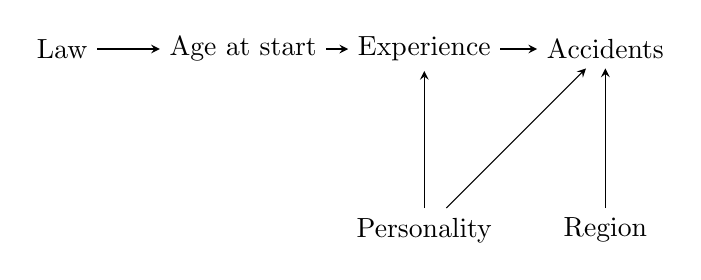
\begin{tikzpicture}[>=stealth, node distance=2.3cm]
	\node (law) {Law};
	\node (age) [right of=law] {Age at start};
	\node (exp) [right of=age] {Experience};
	\node (acc) [right of=exp] {Accidents};
	\node (pers) [below of=exp] {Personality};
	\node (reg) [below of=acc] {Region};

	\draw[->] (law) -- (age);
	\draw[->] (age) -- (exp);
	\draw[->] (exp) -- (acc);
	\draw[->] (pers) -- (exp);
    \draw[->] (pers) -- (acc);
	\draw[->] (reg) -- (acc);
\end{tikzpicture}
\end{center}

Read informally, this says:
\begin{itemize}
	\item The \textbf{Law} constrains the age at which people can start driving.
	\item \textbf{Age at start} influences how much \textbf{Experience} they can accumulate.
	\item \textbf{Experience} influences the risk of \textbf{Accidents}.
	\item \textbf{Personality} (cautious vs reckless) affects both how much \textbf{Experience} people seek and their risk of \textbf{Accidents}.
	\item \textbf{Region} (urban vs rural, road conditions, etc.) also affects \textbf{Accidents}.
\end{itemize}

This kind of diagram helps us see why simply comparing $P(\text{Accidents} \mid \text{Age})$ can be misleading:
\begin{itemize}
	\item Age is entangled with Experience, Personality, and Region.
	\item Changing the Law changes Age, which in turn changes Experience and who drives at all.
\end{itemize}
Causal calculus (Pearl's do-calculus) tells us when and how we can recover $P(Y \mid \operatorname{do}(X=x))$ from purely observational data given such a diagram, and when we cannot.

\subsection{Designing better studies}

Causal models are not only a tool for interpreting existing data; they also guide the \emph{design} of new studies. Given a causal diagram, we can ask:
\begin{itemize}
	\item Which variables must we measure in order to block spurious associations (confounding paths)?
	\item Which variables should we \emph{not} condition on, because they may introduce new biases (colliders)?
	\item Under what conditions can we estimate causal effects from purely observational data?
\end{itemize}

In the Berkeley example, a causal model could tell us that we are missing key variables, such as:
\begin{itemize}
	\item Applicant qualifications (grades, test scores, research experience),
	\item Department climate or reputation for treating women,
	\item Broader social forces shaping field choice.
\end{itemize}
The model would then make explicit that, without additional measurements or assumptions, certain causal questions (e.g., ``Was there discrimination at the department level?'') cannot be answered definitively from the existing data.

\subsection{Reasoning with incomplete data}

Even when we cannot collect more data, causal models still have value. They allow us to:
\begin{itemize}
	\item Enumerate different plausible causal stories consistent with the observed data,
	\item Explore the implications of each story (``If the world worked this way, what would the effect of changing X be?''),
	\item Identify which assumptions are doing the real work in our conclusions.
\end{itemize}
In other words, a causal model acts as a \emph{logic engine} for cause-and-effect reasoning: given explicit assumptions, it yields explicit conclusions, and it clarifies which parts of our reasoning depend on empirical evidence and which parts depend on judgment and prior knowledge.

\section{Summary}

We can now summarize the main points:
\begin{itemize}
	\item Observational data show us how the world \emph{is}, not automatically how it would be if we \emph{changed} something.
	\item Questions about policies or interventions (raising the driving age, changing admissions rules, etc.) are inherently \emph{causal} and require reasoning about $\operatorname{do}(\cdot)$, not just conditional probabilities.
	\item The Berkeley admissions example illustrates how aggregated patterns can reverse when we condition on a relevant variable (department), a phenomenon known as Simpson's paradox.
	\item Observational patterns alone can be compatible with multiple causal explanations (pipeline effects, discrimination at various stages, or both); data without a causal model cannot fully resolve such ambiguities.
	\item Causal models provide a structured way to:
		\begin{itemize}
			\item Distinguish observation from intervention,
			\item Design better studies and decide which variables to measure or control,
			\item Connect domain knowledge and assumptions to concrete, testable implications.
		\end{itemize}
\end{itemize}
In this sense, causal inference is not just an add-on to statistics but a complementary framework that lets us talk rigorously about actions, policies, and the mechanisms that generate the data we see.
